\documentclass[tikz]{standalone}

\usetikzlibrary{matrix.skeleton}

\begin{document}
  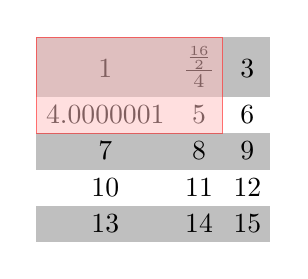
\begin{tikzpicture}
    \matrix (m) [matrix of math nodes,
                 style odd rows on layer={background}{fill=black!25}] {
      1  & \frac{\frac{16}{2}}{4}  & 3  \\
      4.0000001  & 5  & 6  \\
      7  & 8  & 9  \\
      10 & 11 & 12 \\
      13 & 14 & 15 \\
    };
    \fitandstyle{(m-cell-1-1) (m-cell-2-2)}{draw=red, fill=red!25, opacity=0.5}
  \end{tikzpicture}
\end{document}
